\section{Introduction and Scope of Tutorials}
% overall intro from second article works
%OLD:
%WESTPA (The Weighted Ensemble Simulation Toolkit with Parallelization and Analysis; \url{https://westpa.github.io/westpa}) \citep{Zwier2015} is an open-source, highly scalable software framework for carrying out extended-timescale simulations of rare events with rigorous kinetics using the weighted ensemble (WE) strategy \citep{huber_weighted-ensemble_1996}. 
%Key features of WESTPA, written in Python, include (i) a general interface that enables interoperability with any dynamics engine (e.g. Gromacs \citep{gromacs}, Amber \citep{amber}, OpenMM \citep{openmm}); (ii) an optimized, parallel implementation of the WE strategy that exhibits perfect scaling out to >4000 CPU cores; (iii) an effective suite of tools for analysis of the millions of files created by each simulation; (iv) full extensibility for enhancements to simulation protocols and analysis tools; and (v) portability of the software on any Unix-like computing resource, including typical computing clusters and supercomputers. 
%The WESTPA software also includes plugins for using a WE-based string method \citep{Adelman2013} and a WE strategy utilizing hierarchical Voronoi bins (WExplore) \citep{dickson_wexplore_2014}.  
%The WESTPA software package has enabled efficient atomistic simulations of host-guest associations \citep{Zwier2011}, protein binding processes \citep{zwier_efficient_2016, saglam_proteinprotein_2019}, and protein folding \citep{Upendra2019}. 
%This efficiency (relative to standard “brute force” simulations) has been demonstrated to increase exponentially with the effective free energy barrier of the rare event \citep{DeGrave2018}. 


%NEW

The WESTPA (Weighted Ensemble Simulation Toolkit with Parallelization and Analysis) software package \citep{Zwier2015,russo_westpa_2022} is a highly scalable implementation of the weighted ensemble (WE) path sampling strategy \citep{huber_weighted-ensemble_1996,zuckerman_weighted_2017} that has helped transform what is feasible for molecular simulations in the generation of pathways for long-timescale processes (> µs) with rigorous kinetics.
Among these simulations are atomically detailed simulations of protein folding \citep{adhikari_computational_2019}, protein-protein binding \citep{saglam_proteinprotein_2019}, protein-ligand unbinding \citep{lotz_unbiased_2018}, and the large-scale opening of the SARS-CoV-2 spike protein \citep{sztain_glycan_2021}. 
The latter involved the slowest process (seconds-timescale) yet studied for a massive system (one million atoms) using WE simulations. 
As a “bleeding edge” application, these efforts have motivated major upgrades to WESTPA (version 2.0) that enable the sampling of processes at even longer timescales and more streamlined handling of large datasets \citep{russo_westpa_2022}. 
Like its predecessor, WESTPA 2.0 is a Python package that is (i) interoperable, enabling the use of any type of stochastic dynamics simulation (e.g., MD or Monte Carlo simulations) and any model resolution (e.g., atomistic, coarse-grained, non-spatial or spatially resolved systems biology models) \citep{donovan_efficient_2013,donovan_unbiased_2016}; and (ii) extensible, making it straightforward to modify existing modules or create plug-ins in order to support new scientific efforts. 

Here we present a suite of tutorials organized into two groups.
The first four tutorials, presented in the original version of this paper, range in order of difficulty from basic to intermediate, including a tutorial involving the suite of analysis tools. 

The second group of tutorials addresses new features in the major upgrades appearing in the WESTPA 2.0 software package. 
Among these tutorials is one involving the Markovian Weighted Ensemble Milestoning (M-WEM) approach \citep{Ray2022Markovian}, which interfaces the WE strategy with another path sampling method called milestoning \citep{Faradjian2004Computing,West2007Extending}. 
In the final tutorial, we broaden the scope of path sampling to a systems biology application involving a WESTPA plugin for enhancing the efficiency of Monte Carlo simulations using the BioNetGen systems biology package \citep{harris_bionetgen_2016, tapia_mcell-r_2019}. 

For general prerequisites to attempting these tutorials, please see \textbf{Section \ref{intro:prereq}} below.
All files for the tutorials can be found online in the WESTPA Tutorials GitHub repository {\url{https://github.com/westpa/tutorials}}. 
In each tutorial, we outline learning objectives and expected outcomes. 

%These tutorials can also be found online in the WESTPA GitHub repository (\url{https://github.com/westpa/westpa_tutorials/wiki}).
%Learning objectives and expected outcomes are outlined for each tutorial. 
%This set of tutorials is restricted to applications in molecular dynamics (MD) simulations, but WE and WESTPA are applicable to arbitrary stochastic simulations \citep{Donovan2013,Donovan2016,Read2018}.

\subsection{Learning objectives}
After completing the \textbf{Basic Tutorial \ref{tut:nacl-basic}} involving the simulation of Na\textsuperscript{+}/Cl\textsuperscript{-} association, the user should be able to: 
\begin{enumerate}
\item Understand the main simulation directory layout
\item Choose a progress coordinate
\item Choose an appropriate binning scheme
\item Prepare input files
\item Monitor a simulation
\end{enumerate}

After completing the \textbf{Intermediate Tutorial \ref{tut:p53-int}} involving the conformation sampling of a p53 peptide fragment, the user should be able to:
\begin{enumerate}
\item Set up a two-dimensional progress coordinate
\item Monitor this coordinate as the simulation progresses
\item Evaluate whether the binning scheme is effective
\item Combine and create bins “on-the-fly”
\item Store and access auxiliary data
\end{enumerate}

After completing \textbf{Intermediate Tutorial \ref{tut:chig-int}} involving the folding/unfolding of the chignolin mini-protein the user should be able to:
\begin{enumerate}
\item Use brute force simulations to identify appropriate initial and/or target states
\item Obtain the probability flux into the target state of a WESTPA simulation, convert it to a mean rate constant, and interpret the results
\item Approach larger, more biologically relevant events (like protein folding) with a WE-oriented mindset
\end{enumerate}

After completing the \textbf{Analysis Tutorials \ref{tut:analysis-adv}}, the user should be able to:
\begin{enumerate}
\item Calculate progress coordinates using an external analysis suite (MDTraj or MDAnalysis)
\item Automate analysis and interactively explore WE simulation data using the w\textunderscore \verb|ipa| tool
\item Create a movie of how a probability distribution evolves with time
\end{enumerate}

After completing \textbf{Advanced Tutorial \ref{tut:binless}}, which involves the simulation of Na\textsuperscript{+}/Cl\textsuperscript{-} association, the user should be able to:
\begin{enumerate}
  \item Create a customized binless resampler scheme for splitting and merging trajectories based on by k-means clustering using the \verb|BinlessMapper| resampler module;
  \item Initiate a WE simulation from multiple starting conformations;
  \item Combine multiple WE simulations for analysis using the \verb|w_multi_west| multitool;
  \item Perform post-simulation analysis using the \verb|w_crawl| tool.
\end{enumerate}

After completing \textbf{Advanced Tutorial \ref{tut:mem-perm-adv}} involving the simulation of drug membrane permeation, the user should be able to:
\begin{enumerate}
  \item Set up a double membrane bilayer system for permeability studies; 
  \item Use the highly scalable HDF5 framework for more efficient restarting, storage, and analysis of simulations;
  \item Apply the minimal adaptive binning (MAB) scheme.
\end{enumerate}

After completing \textbf{Advanced Tutorial \ref{tut:hamsm-adv}} involving the simulation of ms-timescale protein folding, the user should be able to:
\begin{enumerate}
  \item Apply the haMSM plugin for periodic reweighting of simulations;
  \item Use the \verb|msm_we| package to build an haMSM from WE data;
  \item Estimate the distribution of first passage times.
\end{enumerate}

After completing \textbf{Advanced Tutorial \ref{tut:cust-anal-adv}} involving the creation of custom analysis routines and calculation of rate constants, the user should be able to:
\begin{enumerate}
  \item Access simulation data in a \verb|west.h5| file using the high-level \verb|Run| interface of the \verb|westpa.analysis| Python API and retrieve trajectory data using the \verb|BasicMDTrajectory| and \verb|HDF5MDTrajectory| readers;
  \item Access steady-state populations and fluxes from the \verb|assign.h5| and \verb|direct.h5| data files, convert fluxes to rate constants, and plot the rate constants using an appropriate averaging scheme;
  \item Apply the RED analysis scheme to estimate rate constants from shorter trajectories;
\end{enumerate}

After completing \textbf{Advanced Tutorial \ref{tut:wem-adv}} involving simulations of alanine dipeptide using the M-WEM method, the user should be able to:
\begin{enumerate}
  \item Install the M-WEM software and perform a M-WEM simulation;
  \item Create milestones to define the M-WEM progress coordinate;
  \item Analyze an M-WEM simulation to compute the mean first passage time, committor, and free energy landscape.
\end{enumerate}

After completing \textbf{Advanced Tutorial \ref{tut:bng-adv}} involving rule-based modeling of a gene switch motif using the WESTPA/BNG plugin, the user should be able to:
\begin{enumerate}
  \item Install the WESTPA/BNG plugin and set up a WESTPA/BNG simulation; 
  \item Apply adaptive Voronoi binning, which can be used for both non-spatial and molecular systems; 
  \item Run basic analyses tailored for high-dimensional WESTPA simulations. 
\end{enumerate}

The tutorials will use an array of different dynamics packages to showcase WESTPA’s interoperability. %In each tutorial, all of the required packages and auxiliary programs (for analysis etc.) are freely available and documentation can be readily found online.  The version of each software package is also provided in each tutorial’s “computational requirements” section. 
%
In each tutorial, all of the required software, including the dynamics engine and analysis tools, are freely available with easily-accessible online documentation.
Please note the version of each software package listed in the \textbf{Computational Requirements} section of each tutorial. 

% for single column figure don't include the *
\begin{figure*}[ht]
\centering
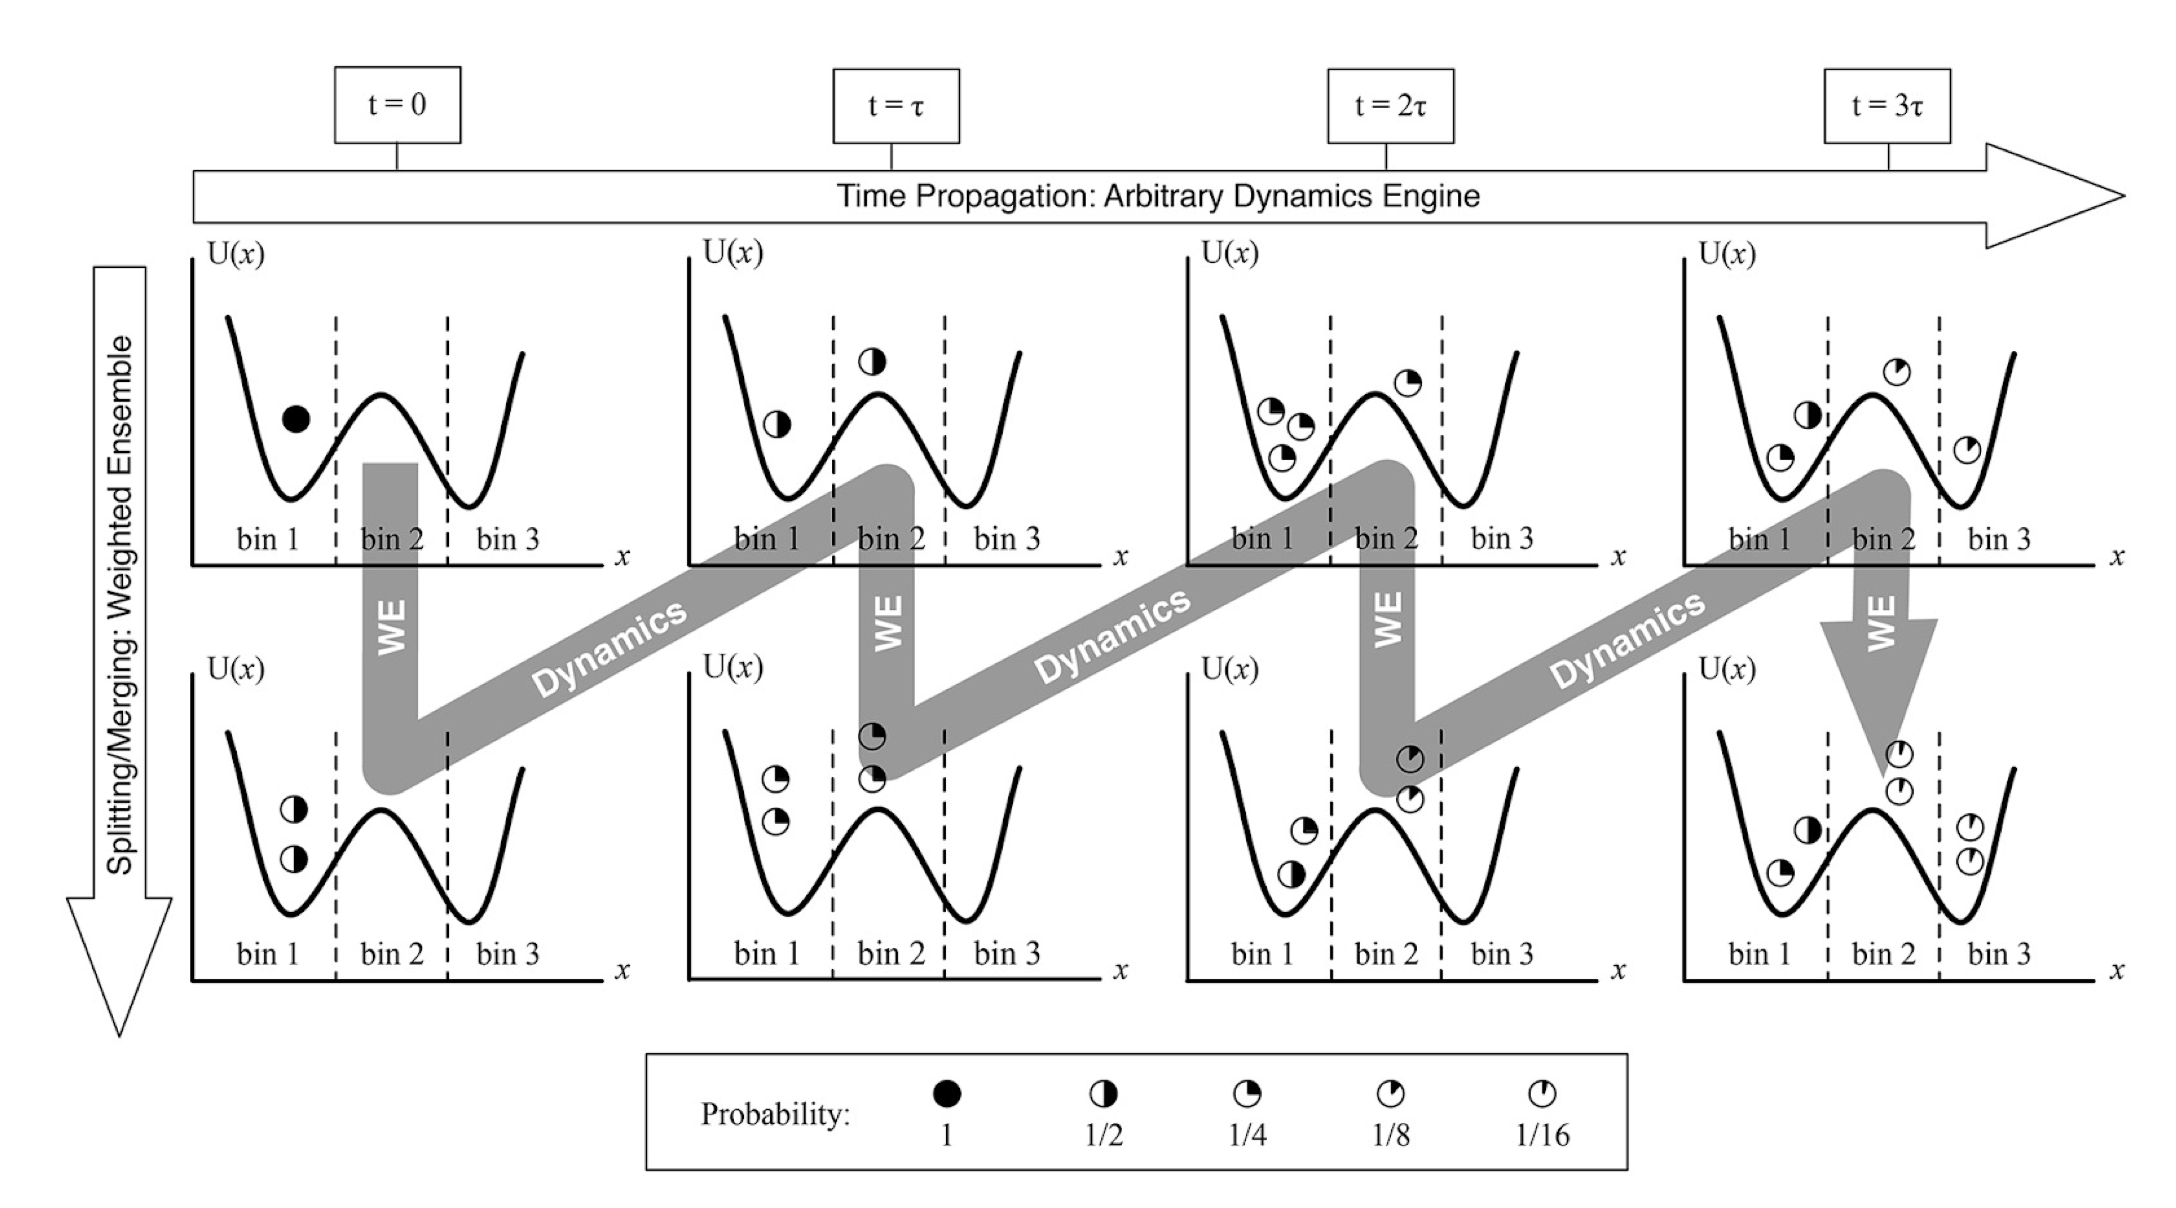
\includegraphics[width=\linewidth]{figure1_WE}
\caption{Overview of the weighted ensemble (WE) strategy \citep{donovan_unbiased_2016}.  WE typically employs bins, demarcated here by dashed vertical lines, to guide a set of trajectories to sample throughout configuration space.
Using only ordinary dynamics---without biasing forces---WE replicates (“splits”) trajectories in unoccupied or under-occupied regions of space and prunes (“merges”) trajectories in over-occupied regions, according to the user-specified allocation scheme which here is a target of two trajectories per bin.
Throughout the process, weights (partially filled circles) are tracked by statistical rules of inheritance that ensure that the overall ensemble dynamics are consistent with non-equilibrium statistical mechanics \citep{zhang_exact_2010}.
Figure adapted with permission from \citep{donovan_efficient_2013}.}
\label{fig:we-overview}
\end{figure*}

%OLD:
\begin{comment}
\subsection{Using WE Concepts in MD Simulation}

The WE strategy organizes an array of MD trajectories strategically in configuration space to target quantities of interest which would not be calculable via standard MD. 
Typical examples are the calculation of pathways and rate constants for conformational and binding processes. 
The overall WE strategy can be embodied in a wide variety of specific algorithms. 
The WESTPA software can be considered a direct descendent of the Huber and Kim algorithm \citep{huber_weighted-ensemble_1996}, although the idea to use trajectory “splitting” and reweighting had been devised decades earlier for research at Los Alamos \citep{KahnHarris1951}.  

As sketched in Figure 1, the essence of WE is to use a statistically unbiased, weighted sample of MD trajectories in such a way that a higher density of trajectories is deployed in regions of configuration space where sampling would otherwise be rare in standard MD. 
These rare regions might be (free) energetic barriers or merely distant regions of configuration space. 
The trajectory weights, which are fundamental to WE, result from the statistical resampling procedures which either prune or replicate trajectories according to rules implemented in WESTPA \citep{huber_weighted-ensemble_1996,Zhang2010,Zwier2015}. 
The rules typically generate trajectory replicates---which will diverge upon additional simulation using a stochastic thermostat or dynamics---in under-sampled regions while pruning trajectories that occur in over-sampled regions.  

Procedurally, WE runs a large number of ordinary, unbiased MD trajectory segments in parallel, with each segment halted and examined after a short interval of time (e.g. 1-100 ps, see Table 1) called $\tau$. 
After each interval, some trajectories are replicated and some are pruned according to user-specified parameters - see below. 
This in turn triggers automated adjustment of the weights to complete the resampling process. 
The remaining trajectories are then continued for another $\tau$ interval.

%%%Fig 1%%%
\begin{figure}
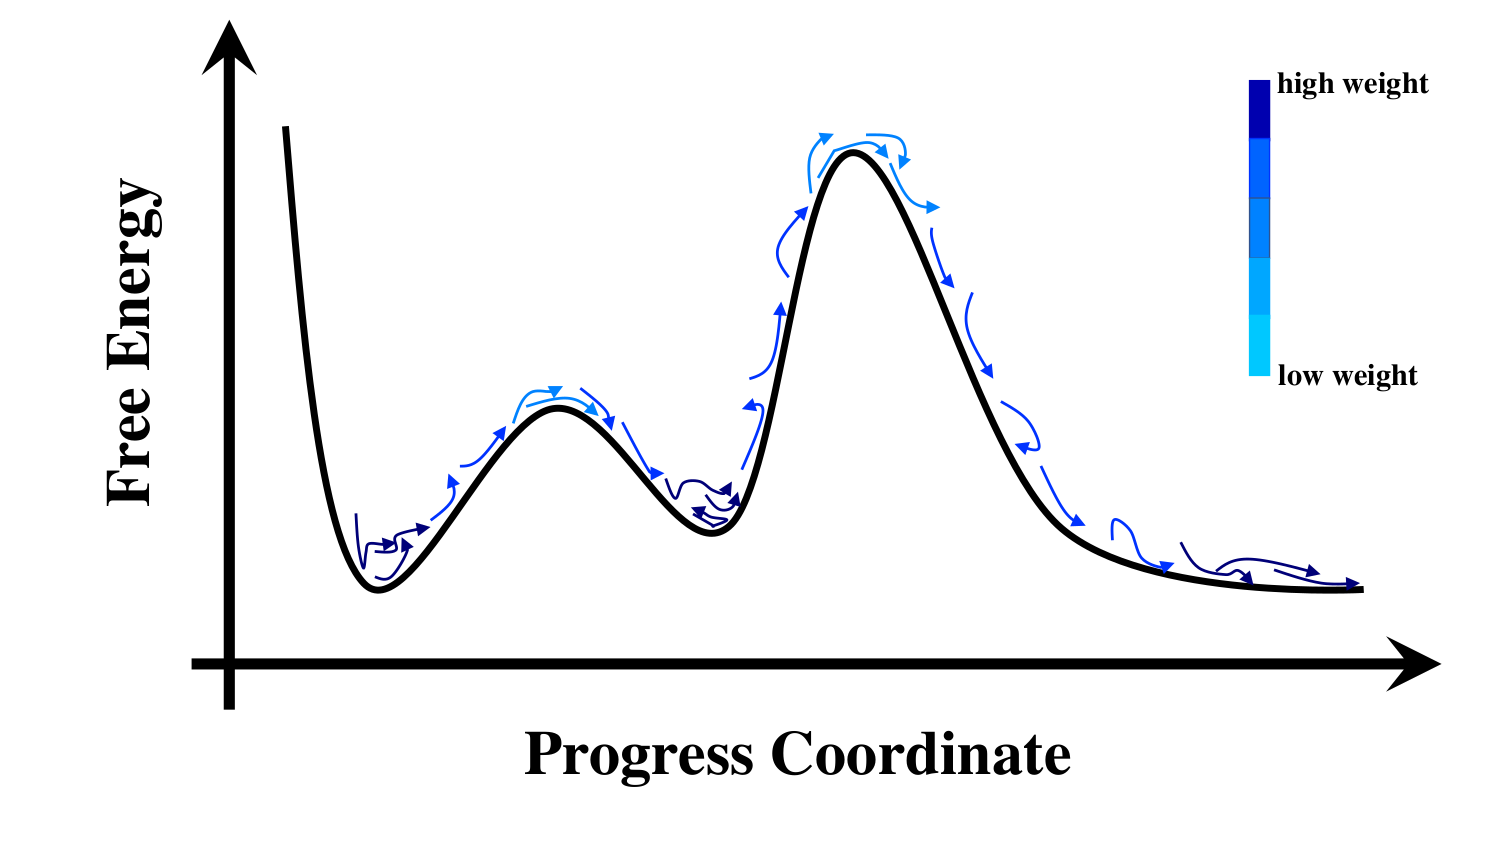
\includegraphics[width=\linewidth]{Figure1.png}
\caption{Weighted ensemble MD simulations. 
Trajectory segments (blue) are fairly evenly distributed in configuration space, and hence enhance sampling of normally undersampled regions of configuration space, such as free energy barriers. 
In this schematic, the free energy or potential of mean force is shown as a function of an arbitrary progress coordinate.
Darker color denotes higher weight trajectories, which will occur at free energy minima and regions initially seeded with trajectories and probability.}
\label{fig:view}
\end{figure}
%%%%%%%%

The rules for resampling trajectories without bias are extremely flexible \citep{Zhang2010} and numerous possibilities are implemented within the WESTPA software. 
Typically, WE simulations rely on “bins,” which are defined regions of configuration space for which the user defines a target number of trajectories \citep{huber_weighted-ensemble_1996}. 
In WESTPA, bins can be constructed from simple one or two-dimensional “progress coordinates”, a hierarchical nesting of bins inside of other bins, Voronoi cells, or the WExplore hierarchical Voronoi strategy \citep{Zwier2015,dickson_wexplore_2014}.
Strictly speaking, it is worth noting that bins are not required to perform WE-like resampling \citep{Dickson2018or19}.

Each WE simulation ultimately yields an ensemble of trajectories, from which different types of information can be extracted. 
Each trajectory which makes a full transition between states of interest, say from A to B, yields an ordered set of configurations which can be analyzed for structural changes and for the sequence of events. 
The full weighted ensemble of trajectories, if clustered into pathway groups, can provide information on the relative importance of different pathways \citep{Ernesto2019}. 
If WE was performed with a “recycling” condition where trajectories reaching B are fed back to A, then the rate constant for the process can be estimated from the probability flux arriving to state B if the simulation achieves steady state and hence constant flux \citep{Divesh2010,ZuckermanChong2017}.
If a WE simulation does not achieve steady state, it is still possible in principle to estimate rate constants using a non-Markovian analysis, also called a history-augmented Markov State Model \cite{Ernesto2014,Upendra2019,copperman_accelerated_2020}.
\end{comment}


%NEW:

\subsection{The Weighted Ensemble Strategy}

WE is a highly-parallel path sampling strategy for generating rare events, for studying non-equilibrium steady states, and less commonly, for studying equilibrium properties. 
At heart, it is a simple and flexible strategy which is agnostic to system type and which therefore lends itself to numerous applications and optimizations. 
The properties of WE, including strengths and limitations, have been reviewed in detail before \citep{zuckerman_weighted_2017}, although improvements continue to be developed \citep{donyapour_revo_2019, copperman_accelerated_2020, torrillo_minimal_2021, degrave_red_2021, aristoff_optimizing_2020}. 
Here, we briefly review key aspects of WE.

\textbf{The Basic WE Procedure.} See \textbf{Figure \ref{fig:we-overview}}. 
WE orchestrates multiple trajectories---each assigned a weight---run in parallel by stopping them at regular time intervals of length $\tau$ (typically a large multiple of the underlying simulation time step), examining the trajectories, and restarting a new set of trajectories. 
The new trajectories are always continuations of the existing set, but some trajectories may not be continued (they are “pruned”) and others may be replicated. 
Discontinued trajectories result from probabilistic “merge” events where a continued trajectory absorbs the weight of one that is pruned. 
Replicated trajectories are said to be “split” with the original weight shared equally among the copies. 
Usually bins in configuration space are used to guide split and merge events based on a target number of trajectories for each bin, but any protocol---including binless strategies highlighted below---may be used for this purpose.
Regardless of the resampling protocol, a “recycling” protocol often is used whereby events reaching a user-specified target state are re-initiated according to a specified distribution of start states \citep{bhatt_steady-state_2010}.
This recycling protocol focuses all sampling on a single direction of a process of interest and has valuable properties as noted below.

\textbf{WE is Resampling, and Hence Unbiased.} The simple steps defining WE simulations stem from its basis as a statistical “resampling” procedure \citep{zhang_exact_2010}. 
The split/merge steps generate a statistically equivalent (re)sample of an initial trajectory set by increasing/reducing trajectory density in some regions of configuration space at a given time, using weight adjustments to maintain the underlying trajectory distribution. 
The trajectory set is therefore unbiased at all times, i.e., average time-dependent observables derived from many WE runs will match the average of a large number of conventional simulations without splitting or merging events \citep{zhang_exact_2010}. 
Furthermore, the distributions of transition path times (“barrier crossing times”) from WE runs match those from converged conventional simulations, and can be generated in orders of magnitude less computing time \citep{zwier_efficient_2011, zheng_simulating_2007}. 
The lack of bias in the dynamics of WE runs holds true regardless of whether recycling is employed.

\textbf{Observables and Ensembles Sampled by WE.} WE can yield transient and/or steady-state observables. 
When recycling is not used, WE provides pathways, i.e., sequences of conformations in a transition and the frequencies of those sequences, in addition to time-dependent observables as the system relaxes to equilibrium, e.g., the probability of a given event at a given time after initiation in the chosen starting state.
Complex systems are unlikely to relax fully to equilibrium during a WE simulation. 
With a recycling protocol, the system will not relax to equilibrium but instead to a non-equilibrium steady state (NESS) that has steady probability flow from initial to target state. 
If reached, the NESS provides a simple mechanism for computing rate constants via the Hill relation \citep{bhatt_steady-state_2010}. 
However, although relaxation to a NESS can be considerably faster than relaxation to equilibrium \citep{copperman_transient_2019,zuckerman_discrete-state_nodate}, the process may be too slow for WE to reach NESS on practical timescales, motivating the haMSM approach \citep{adhikari_computational_2019,copperman_accelerated_2020} described below.

\textbf{Resampling Introduces Correlations, which Increase Variance.} WE has intrinsic limitations, like any method \citep{chong_path-sampling_2017}, and it is essential to understand them. 
Most fundamentally, splitting and merging introduce correlations into the sampled trajectory ensemble that could decrease its information content. 
These stem primarily from splitting events: multiple trajectories share an identical history up to the time of the split event and hence do not contribute fully independent information to any observable.
These correlations, in turn, can lead to large run-to-run variance \citep{adhikari_computational_2019} because the trajectory ensemble in each WE run results from a relatively small number of “parent” trajectories which have been split repeatedly.
This variance is addressed to some extent by the iterative haMSM protocol described below, and more directly by ongoing mathematical optimizations noted below.  
Importantly, correlations within WE ensembles lead to significant challenges in quantifying uncertainty \citep{zuckerman_weighted_2017,mostofian_statistical_2019}.

\textbf{Ongiong Efforts at Optimization and Variance Reduction.} Because WE is unbiased so long as a correct resampling protocol is used \citep{zhang_exact_2010}, there is an opportunity to reduce the run-to-run variance noted above by improved resampling procedures. 
In the context of binned WE simulations, both the construction of bins and the number of trajectories per bin can be optimized based on a recently developed mathematical formulation \citep{aristoff_analysis_2018, aristoff_optimizing_2020} or based on heuristics \citep{torrillo_minimal_2021}. 
Bins do not need to be kept static over time \citep{zhang_exact_2010,torrillo_minimal_2021}. 
Optimization approaches are actively being studied and incorporated into WESTPA as appropriate.

\textbf{WE Cannot Solve Every Problem.} Despite its great strengths and highly notable achievements \citep{lotz_unbiased_2018, sztain_glycan_2021, adhikari_computational_2019}, users should not assume WE can tackle any problem.
Independent of the correlation/variance issues noted above, certain systems will remain too complex for WE given current hardware and algorithms.
In every system, there is a minimum transition path time t\textsubscript{TP} (also called t\textsubscript{b}) \citep{zuckerman_transition_2002, zhang_efficient_2007} for physically realistic events which sets an absolute requirement on sampling required: in a WE run, a set of trajectories exceeding the minimum t\textsubscript{TP} must be generated, which may be a prohibitive cost.
Additionally, even if the necessary computing resources are available, current binning and resampling strategies might not be sufficient to generate events of interest. 
And finally, even if events of interest are generated, the sampled trajectories may be insufficient for producing observables of interest such as a reliable estimate of the rate constant.

%OLD:
\begin{comment}
\subsection{Prerequisites}

\subsubsection{Background Knowledge and Experience}

The WESTPA software is not intended for total beginners in molecular simulation. 
A prerequisite for all of WESTPA tutorials presented here is that users already have extensive experience with running standard molecular dynamics (MD) simulations using the underlying dynamics engine of interest (Amber, Gromacs, OpenMM, etc.). 
In fact, we recommend running multiple short, standard simulations prior to applying the WE strategy in order to (i) ensure that the system is prepared and the dynamics are propagated according to best practices (e.g., see \citep{Mobley2019}), (ii) identify potential progress coordinates and other observables that may be worth monitoring during the WE simulation, (iii) determine an initial definition of the target state, and (iv) estimate storage needs for your eventual WE simulation and the ns/day that can be generated for your system. 
It is also important to identify sources of validation for your simulation (e.g., from experiment and/or standard simulations) and to be familiar with the estimation of statistical uncertainty in the computed observables, including those used for validation (\citep{Grossfield2019}). 
We highly recommend that new users read the WE overview (\url{https://westpa.github.io/westpa/overview.html}) as well as a recent review article \citep{ZuckermanChong2017}. 
In addition, new users are encouraged to search the WESTPA mailing list (\url{https://groups.google.com/forum/#!forum/westpa-users}) for possible solutions or to submit questions/issues to the mailing list.
\end{comment}

%NEW
\subsection{Prerequisites and Computing Requirements}
\label{intro:prereq}

\textbf{Background Knowledge and Experience.} 
The WESTPA software is not intended for total beginners in molecular simulation. 
%All tutorials here are at the advanced level. 
%Thus, a prerequisite for these tutorials is completion of the Basic and Intermediate WESTPA tutorials \citep{bogetti_suite_2019}, which have been updated for use with WESTPA version 2.0 ({\url{https://github.com/westpa/westpa_tutorials}}). 
Users should already have extensive experience running conventional simulations using the underlying dynamics engine of interest (Amber \citep{case_amber_2022}, OpenMM \citep{eastman_openmm_2017}, BioNetGen \citep{harris_bionetgen_2016}, etc.). 
Prior to applying the WE strategy to their own systems, we suggest that users run multiple conventional simulations to (i) ensure that the preparation of the system and propagation of dynamics is according to best practices (e.g., see \citep{braun_best_2019}), (ii) identify potential progress coordinates and initially define the target state, and (iii) estimate the ns/day on a single CPU/GPU for your system and storage needs for the full-scale WE simulation. 
We highly recommend that new WESTPA users read this review article \citep{zuckerman_weighted_2017} and this introduction to non-equilibrium physics of trajectories \citep{zuckerman_gentle_2021}. 
It is also important to identify sources of validation for your simulation (e.g., from experiment and/or standard simulations) and to be familiar with the estimation of statistical uncertainty in the computed observables, including those used for validation \citep{Grossfield2019}. 
%OLD:
\begin{comment}
\subsubsection{Software Requirements}

The WESTPA software requires Python and a number of standard Python scientific computing packages. 
All required software is available through the Anaconda Python distribution, which also provides the preferred mechanism for obtaining and installing WESTPA itself. 
The software can be used on any Unix operating system, including academic clusters and supercomputers. 
The installation of WESTPA is streamlined by an Anaconda conda install recipe that enables WESTPA and all software dependencies to be installed at the same time.

In addition, WESTPA will require interfacing with an external dynamics engine in order to run WE simulations.  Examples of dynamics engines that can be used (all free of charge), and the versions used are included before each tutorial in this manuscript.
\end{comment}

\textbf{Software Requirements.} 
The WESTPA 2.0 software is a standard Python package that can be used on any Unix operating system. 
The software requires Python versions $\geq$3.8 and a number of standard Python scientific computing packages. 
We recommend installing WESTPA either as a PyPI or conda package using miniconda. 
Both packages provide all required software dependencies and can be installed using one-line commands: (1) \verb|python -m pip install westpa| or (2) \verb|conda install -c conda-forge westpa|. 
Note that it is a best practice to install WESTPA into an isolated virtual or conda environment, along with the dependencies specific to your project. 
Due to the use of the MDTraj Python library with the WESTPA 2.0 HDF5 framework, certain modifications to the installation procedure are required for running WESTPA 2.0 on ppc64Ie architectures (e.g., TACC Longhorn or ORNL Summit supercomputers; see {\url{https://github.com/westpa/westpa/wiki/Alternate-Installation-Instructions}}). 

WESTPA 2.0 is designed to be interoperable with any dynamics engine, requiring an external dynamics engine to propagate the dynamics in a WE simulation.
Please see the prerequisite sections of each tutorial for additional software requirements that are specific to that tutorial.

\begin{comment}
%OLD:
\subsubsection{Hardware Requirements}

The highly scalable WESTPA software is particularly well-suited for high-performance computing (HPC) clusters, including those at academic institutions or supercomputing centers. 
Much of the computing effort is independent (i.e. highly parallelizable) with only a small amount of data being transferred to a central process at the end of each WE iteration. 
Furthermore, the amount of memory per computing node need only be sufficient for the underlying dynamics engine, e.g., \textasciitilde 1 GB per CPU core for atomistic MD simulations. 

The two major computing hardware considerations for large-scale WESTPA simulations are (i) the number of available processors, and (ii) the amount of disk storage in the scratch (working) space. 
Further details about these requirements are provided below. 

\textbf{Number of Processors.} WESTPA can be run on even a single processor, but the ideal scenario is to use the same number of processors — all with the same processor speed — as the number of trajectories you are simultaneously running at any point in time; in this way, all trajectories that are being run can be completed at the same time. 
If the ideal number of processors is not available, we suggest requesting a number by which the number of trajectories at any point in time is divisible. 
These are not strict requirements, but following these guidelines will ensure the most economical use of computer time possible.

\textbf{Storage Requirements.} To estimate the storage requirement for your WE simulation, we suggest running a single MD simulation for length $\tau$, estimating the maximum number of trajectories you will generate for any WE iteration (number of bins multiplied by number of trajectories per bin), and estimating the number of WE iterations you will need to converge the observable of interest. 
This results in the maximum total number of trajectories per simulation, which can be used to estimate the total storage requirements (both number of files and aggregate storage space). 
Ideally, the scratch space of your computing cluster should be sufficiently large to temporarily store the entire simulation, which makes the analysis easier in the not-unlikely event you need to reanalyze each trajectory. 
Regardless of your estimate, having an off-cluster storage option that can store the simulation in case you need to extend the simulation further on the cluster would be ideal. 
Also, make sure that you are not exceeding any limits on the total number of files a user can have on your computing cluster. 

As an example, we present the hardware requirements of our largest-scale WESTPA simulation to date, which involved a protein-protein binding process in explicit solvent. 
To enable convenient analysis of this simulation, the scratch directory of a computing cluster would ideally allow for 15 TB of disk space to store trajectory coordinates for the entire system, including explicit water molecules, checkpoint files for continuing trajectories, and other files required for analysis. 
If the scratch space is much less than this amount (e.g. 2 TB), we recommend separately tarring and archiving each WE iteration, keeping the last five WE iterations untarred, and moving the archived files to local storage. 
This strategy enables one to restart a WE simulation from the last few iterations if necessary. 
We realize that this protein-protein binding simulation is an extreme use case, but nonetheless, this scenario highlights the importance of allocating the necessary storage space for more typical use cases. 

We note that most distributed storage filesystems used on large clusters (e.g. Lustre or GPFS) do not distribute metadata (file size, modification time, etc.) processing, and this centralized treatment of metadata can become a "choke point" for WESTPA simulations. 
In the worst case, a poorly-configured WESTPA simulation can result in denial of service to other users. 
There are no viable alternative file systems at this time. 
Fortunately, a simple remedy exists. The burden of running WESTPA simulations on these distributed filesystems can be substantially reduced by using the full pathnames to all executables called by any WESTPA process (for example, writing \verb|/usr/bin/awk| instead of simply \verb|awk|).

\subsubsection{Running WESTPA on a Computing Cluster}

Prior to running full-blown WESTPA simulations on your desired computing cluster, it is advisable to consult with the system administrator about how best to run your simulation on the cluster. 
In addition, test simulations consisting of a few WE iterations should be run using the development queue to gauge if the I/O is too frequent for the cluster and to optimize the execution of your simulation (see Table 1 for examples of computing resources that have been suitable for various WE applications). 
Sample shell scripts for executing WESTPA simulations on various computing resources have been provided for the Intermediate Tutorial (Section 6.2) on GitHub. 
\end{comment}

%\hl{update Table 1?  delete?}
\begin{table*}
\label{intro:table1}
\caption{WE parameters used for notable applications in the literature. 
The asterisk (*) indicates an application with I/O operations that is too frequent for supercomputers and gaming GPUs.}
\centering
\begin{tabular}{ | p{0.11\linewidth} | p{0.30\linewidth} | p{0.30\linewidth} | p{0.17\linewidth} |}
\hline
\textbf{Rare-event process} & 
\textbf{System and size} & 
\textbf{WE Parameters} & 
\textbf{Suitable computing resources} \\
\hline
millisecond protein 

folding \citep{mostofian_statistical_2019} & 
NTL9 protein in generalized Born (GB) implicit solvent with low and high 

solvent viscosity (collision frequency of 5 ps\textsuperscript{-1} and 80 ps\textsuperscript{-1}, respectively): 

627 atoms & 
1D progress coordinate: C\textsubscript{$\alpha$} RMSD from the folded structure.

Binning: 53 bins, that are finely spaced for near-folded structures (35 bins for 1.0 \AA{} < RMSD < 4.4 \AA) and more coarsely spaced for more unfolded structures: 

(12 bins for 4.4 \AA{} < RMSD < 6.6 \AA{} and 

5 bins for 6.6 \AA{} < RMSD < 10.2 \AA).

$\tau$ = 10 ps; 1200 WE iterations;

4 trajectories/bin
& Professional-graphics-programming GPUs\textsuperscript{*} (e.g. NVIDIA Quadro RTX 5000) \\
\hline
peptide-protein association \citep{zwier_efficient_2016} & 
p53 peptide/MDM2 protein in GB/SA implicit solvent: 1685 atoms & 
2D progress coordinate: heavy-atom RMSD of p53 peptide relative to its MDM2-bound conformation following alignment on (i) MDM2 and (ii) itself. 

Binning: 16 bins with 0.5 \AA{} widths along the p53-aligned RMSD and widths ranging from 0.2 to 2 \AA{} for the MDM2-aligned RMSD. 

$\tau$ = 50 ps; 396 WE iterations;

8 trajectories/bin & 
1600 CPU cores on a supercomputer (e.g. PSC’s Bridges-2) or 16 GPUs (e.g. NVIDIA A100 GPUs) \\
\hline
protein-protein association \citep{saglam_proteinprotein_2019} & 
barnase/barstar proteins in explicit solvent: >100,000 atoms & 
2D progress coordinate: (i) heavy-atom RMSD of barstar residues D35 and D39 after alignment on barnase, and (ii) minimum protein-protein separation distance.  
D35 and D39 are the barstar residues that become the most buried upon binding barnase.

$\tau$ = 20 ps; 650 WE iterations

Binning: 72 bins with coarsely spaced bins every 1 \AA{} from 10 to 60 \AA{} and more finely spaced bins every 0.5 \AA{} from 0 to 10 \AA{} along the RMSD coordinate; two bins along the distance coordinate separated by a bin boundary at 5 \AA{}; fixed total number of trajectories (1600)& 
1600 CPU cores on a supercomputer (e.g. PSC’s Bridges-2) or 16 GPUs (e.g. NVIDIA A100 GPUs) \\
\hline
\end{tabular}
\end{table*}

%NEW:
\textbf{Hardware Requirements.} Like its predecessor, WESTPA 2.0 is highly-scalable on CPUs/GPUs, making optimal use of high-performance computing (HPC) clusters available at academic institutions or supercomputing centers. 
Memory requirements are dependent on the underlying dynamics engine, e.g., \textasciitilde1 GB per CPU core (or GPU) for atomistic MD simulations. 
Users should refer to the best practices of their dynamics engine of choice to determine the optimal allocation of resources for each CPU/GPU. 
The most efficient way to run WESTPA is to use a computing resource that provides the user with a number of CPUs/GPUs---all the same processor speed---that either matches the number of trajectories per WE iteration or a number by which the number of trajectories at any point in time is evenly divisible. 
WE can nevertheless run on heterogeneous hardware (different processor or memory bus speeds) or with trajectory counts that do not divide evenly onto CPUs/GPUs, but this scenario decreases efficiency as some processors are inevitably idle for at least a portion of the overall runtime.

Users can estimate the approximate storage space required for their project by taking the product of the following: (i) amount of disk space required for storing data from one trajectory segment of length $\tau$, (ii) the maximum number of trajectories per WE iteration, and (iii) the total number of WE iterations required to generate a reasonable maximum trajectory length. 
To optimize the use of storage space, we recommend that users tar up trajectory files into a single file for each WE iteration and remove coordinates of the system that are not of primary interest (e.g., solvent coordinates for certain processes). 
We note that the WESTPA 2.0 HDF5 framework dramatically reduces the storage space required for trajectory coordinates by consolidating the data from millions of small trajectory files into a relatively small number of larger HDF5 files, reducing the large overhead from the file system that results from the storage of numerous small trajectory files. 
By doing so, the HDF5 framework also alleviates potential I/O bottlenecks when a large amount of simulation files are written after each WE iteration. 